\documentclass[tikz,border=5pt]{standalone}
\usepackage[utf8]{vietnam}
\usepackage{amsmath,amssymb}
\usepackage{tikz}

\begin{document}
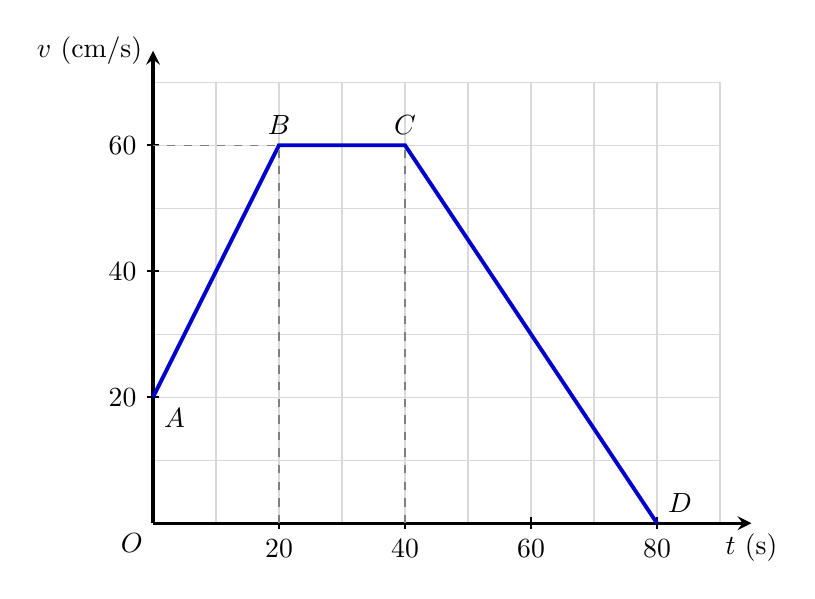
\begin{tikzpicture}[xscale=0.08, yscale=0.08, thick, >=stealth]
	% Hệ lưới tọa độ ô chia
	\draw[lightgray!60, thin, step=10] (0,0) grid (90,70);
	% Hệ trục tọa độ chính
	\draw[->, line width=1.2pt] (0,0) -- (95,0) node[below] {$t\text{ (s)}$};
	\draw[->, line width=1.2pt] (0,0) -- (0,75) node[left] {$v\text{ (cm/s)}$};
	\node[below left] at (0,0) {$O$};
	% Các vạch chỉ số mốc chính trục ngang
	\foreach \x in {20, 40, 60, 80} {
		\draw (\x, 1) -- (\x, -1) node[below] {$\x$};
	}
	% Các vạch chỉ số mốc chính trục đứng
	\foreach \y in {20, 40, 60} {
		\draw (1, \y) -- (-1, \y) node[left] {$\y$};
	}
	% Vẽ các đoạn gấp khúc đồ thị động học
	\draw[blue!80!black, line width=1.4pt] (0,20) node[below right, black] {$A$} -- (20,60) node[above, black] {$B$} -- (40,60) node[above, black] {$C$} -- (80,0) node[above right, black] {$D$};
	% Các đường dóng nét đứt phụ trợ
	\draw[dashed, thin, gray] (20,0) -- (20,60) -- (0,60);
	\draw[dashed, thin, gray] (40,0) -- (40,60);
	\foreach \p in {(0,20), (20,60), (40,60), (80,0)} {
		\fill[black] \p circle (1.8pt);
	}
\end{tikzpicture}
\end{document}
